\documentclass{beamer}
\usepackage{graphicx}
\usepackage{amsmath, esint}

\usepackage{ragged2e}
\usepackage{tikz}
\usetikzlibrary{arrows,shapes}

\usepackage{listings}
\lstset{escapeinside={@(}{)@}}
\usepackage{algorithm}
\usepackage{algorithmic}

\usepackage{minted}
\usepackage{xcolor} 
\definecolor{LightGray}{gray}{0.975}

\usepackage{amssymb}

\def\ojoin{\setbox0=\hbox{$\bowtie$}%
  \rule[-.02ex]{.25em}{.4pt}\llap{\rule[\ht0]{.25em}{.4pt}}}
\def\leftouterjoin{\mathbin{\ojoin\mkern-5.8mu\bowtie}}
\def\rightouterjoin{\mathbin{\bowtie\mkern-5.8mu\ojoin}}
\def\fullouterjoin{\mathbin{\ojoin\mkern-5.8mu\bowtie\mkern-5.8mu\ojoin}}

%\usetheme{Warsaw}
\usefonttheme{serif} 

\title[Chapter 4]{Database System Concepts, $7^{th}$ Edition \\ Chapter 4: Intermediate SQL}
\author{Silberschatz, Korth and Sudarshan}
\date{\today}

\setbeamertemplate{navigation symbols}{}%remove navigation symbols

\defbeamertemplate*{footline}{shadow theme}
{%
  \leavevmode%
  \hbox{\begin{beamercolorbox}[wd=.5\paperwidth,ht=2.5ex,dp=1.125ex,leftskip=.3cm plus1fil,rightskip=.3cm]{author in head/foot}%
    \usebeamerfont{author in head/foot} Database System Concepts \hfill \insertshorttitle
  \end{beamercolorbox}%
  \begin{beamercolorbox}[wd=.5\paperwidth,ht=2.5ex,dp=1.125ex,leftskip=.3cm,rightskip=.3cm plus1fil]{title in head/foot}%
    \usebeamerfont{title in head/foot} \hfill \insertframenumber\,/\,\inserttotalframenumber%
  \end{beamercolorbox}}%
  \vskip0pt%
}

\AtBeginSection[]
{
     \begin{frame}<beamer>
     \frametitle{Plan}
     \tableofcontents[currentsection]
     \end{frame}
}

\newcommand{\toRight}[1]{
    \begin{FlushRight}
        {\tiny #1}
    \end{FlushRight}
} % Align to right

\begin{document}

\frame{\titlepage}

\begin{frame}{Database System Concepts}
    \centering
    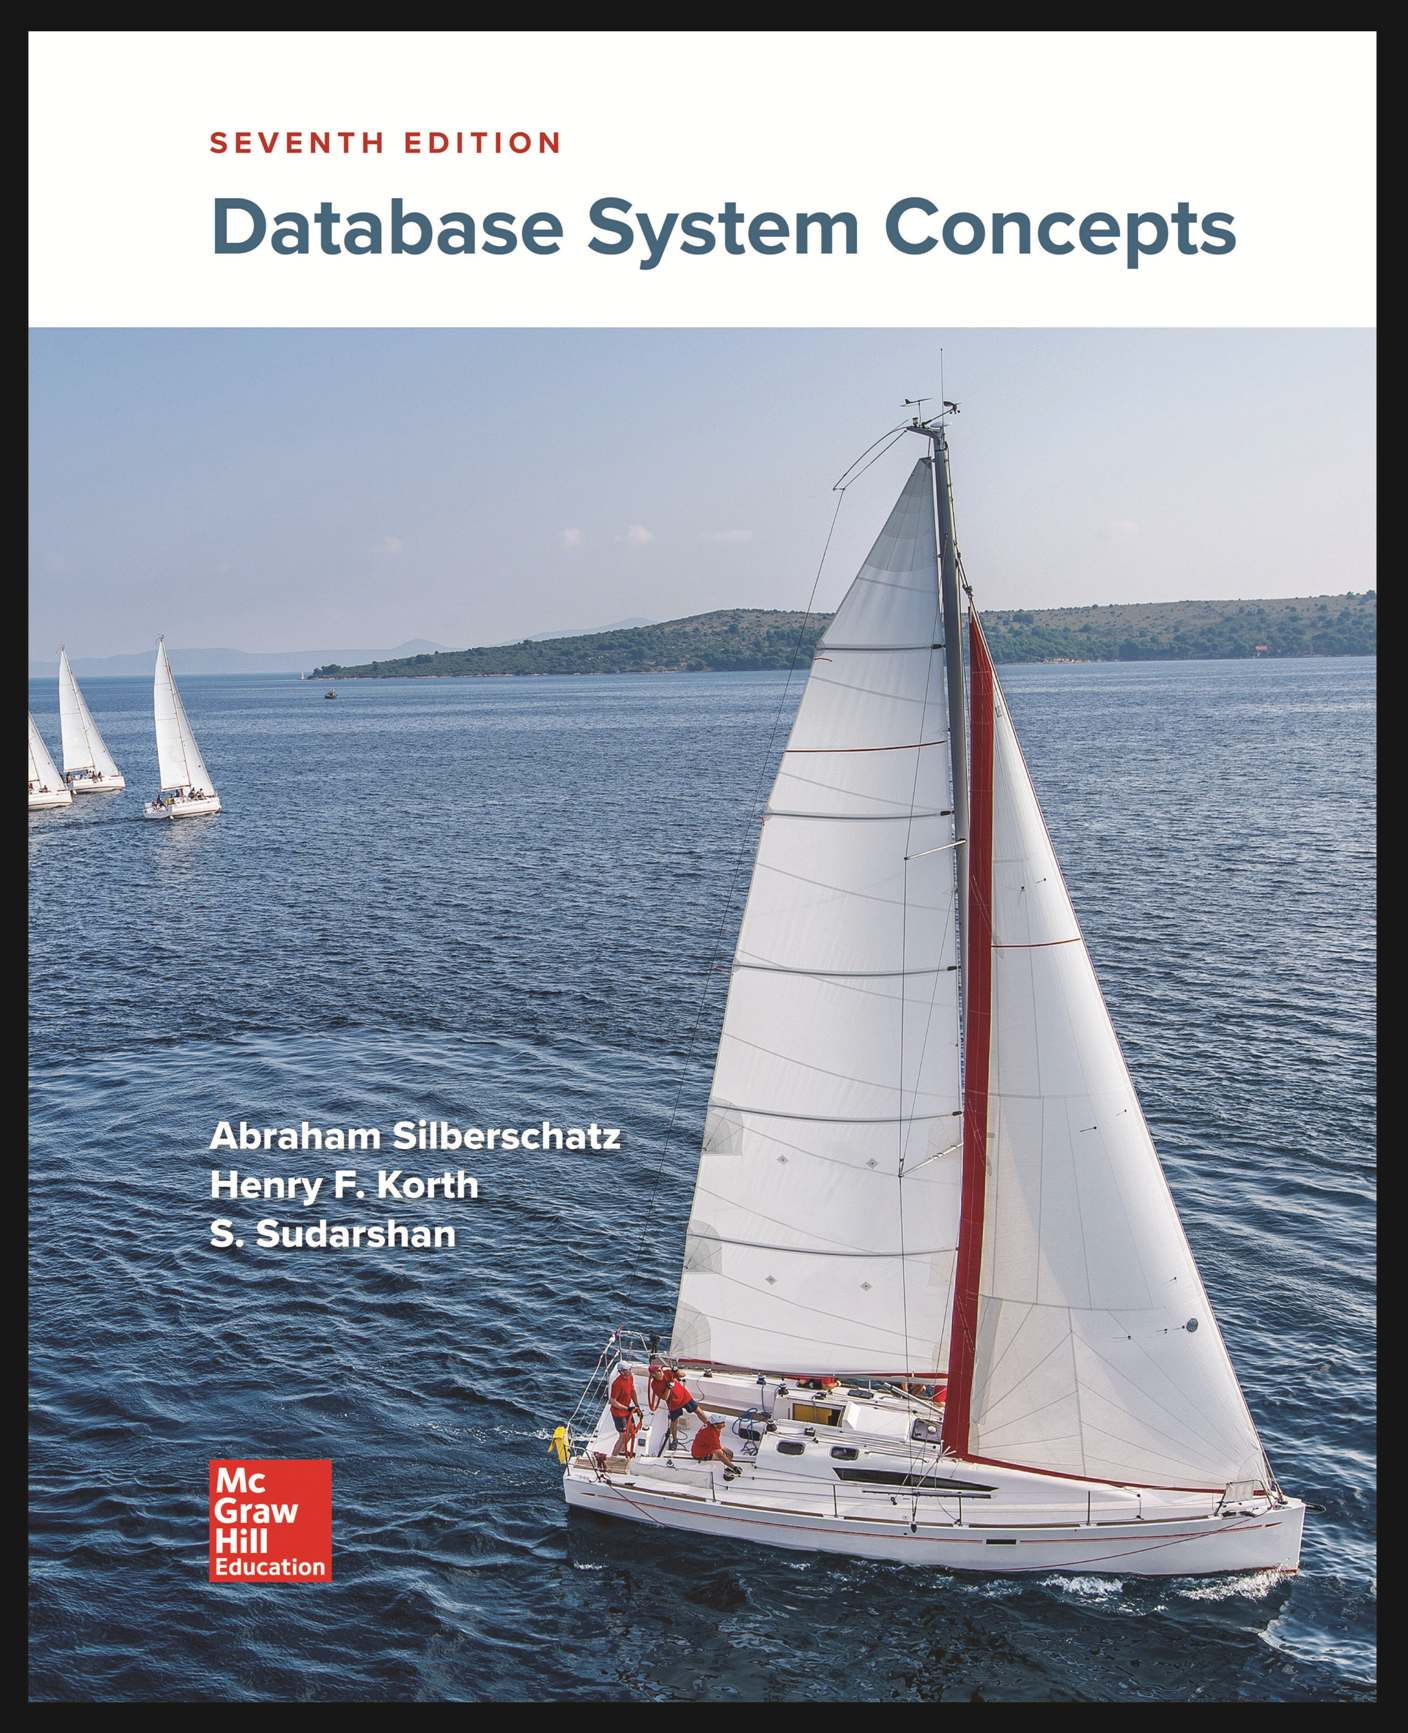
\includegraphics[width=0.5\textwidth]{figures/book_cover.jpg} \\
    \vspace{5mm}
    {
        \tiny
        Content has been extracted from \textit{Database System Concepts}, Seventh Edition, by Silberschatz, Korth and Sudarshan. Mc Graw Hill Education. 2019.\\
        Visit \url{https://db-book.com/}.\\
    }
\end{frame}

\section{Join Expressions}

\begin{frame}{Joined Relations}
    \begin{itemize}
        \item Join operations take two relations and return as a result another relation.
        \item A join operation is a Cartesian product which requires that tuples in the two relations match (under some condition). It also specifies the attributes that are present in the result of the join.
        \item The join operations are typically used as subquery expressions in the \texttt{FROM} clause.
        \item Three types of joins:
        \begin{itemize}
            \item Natural join
            \item Inner join
            \item Outer join
        \end{itemize}
    \end{itemize}
\end{frame}

\begin{frame}[fragile]{Natural Join in SQL}
    \begin{itemize}
        \item Natural join matches tuples with the same values for all common attributes, and retains only one copy of each common column.
        \item For all students in the university who have taken some course, find their names and the course ID of all courses they took.
        \begin{minted}
        [tabsize=4, obeytabs, frame=lines, framesep=2mm, baselinestretch=1.2, bgcolor=LightGray, fontsize=\footnotesize, linenos]{sql}
        SELECT
            name, course_id
        FROM
            students, takes
        WHERE
            student.ID = takes.ID;
        \end{minted}
    \end{itemize}
\end{frame}

\begin{frame}[fragile]{Natural Join in SQL}
    \begin{itemize}
        \item Same query in SQL with ``natural join'' construct.
        \begin{minted}
        [tabsize=4, obeytabs, frame=lines, framesep=2mm, baselinestretch=1.2, bgcolor=LightGray, fontsize=\footnotesize, linenos]{sql}
SELECT
    name, course_id
FROM
    student NATURAL JOIN takes;
        \end{minted}
    \end{itemize}
\end{frame}

\begin{frame}[fragile]{Natural Join in SQL (Cont.)}
    \begin{itemize}
        \item The \texttt{FROM} clause can have multiple relations combined using natural join:
        \begin{lstlisting}[language=SQL]
SELECT @($A_1, A_2, \ldots, A_n$)@
FROM @($r_1$)@ 
    NATURAL JOIN @($r_2$)@ 
    NATURAL JOIN @($\ldots$)@ 
    NATURAL JOIN @($r_n$)@
WHERE @($P$)@;
        \end{lstlisting}
    \end{itemize}
\end{frame}

\begin{frame}{Student Relation}
    \centering
    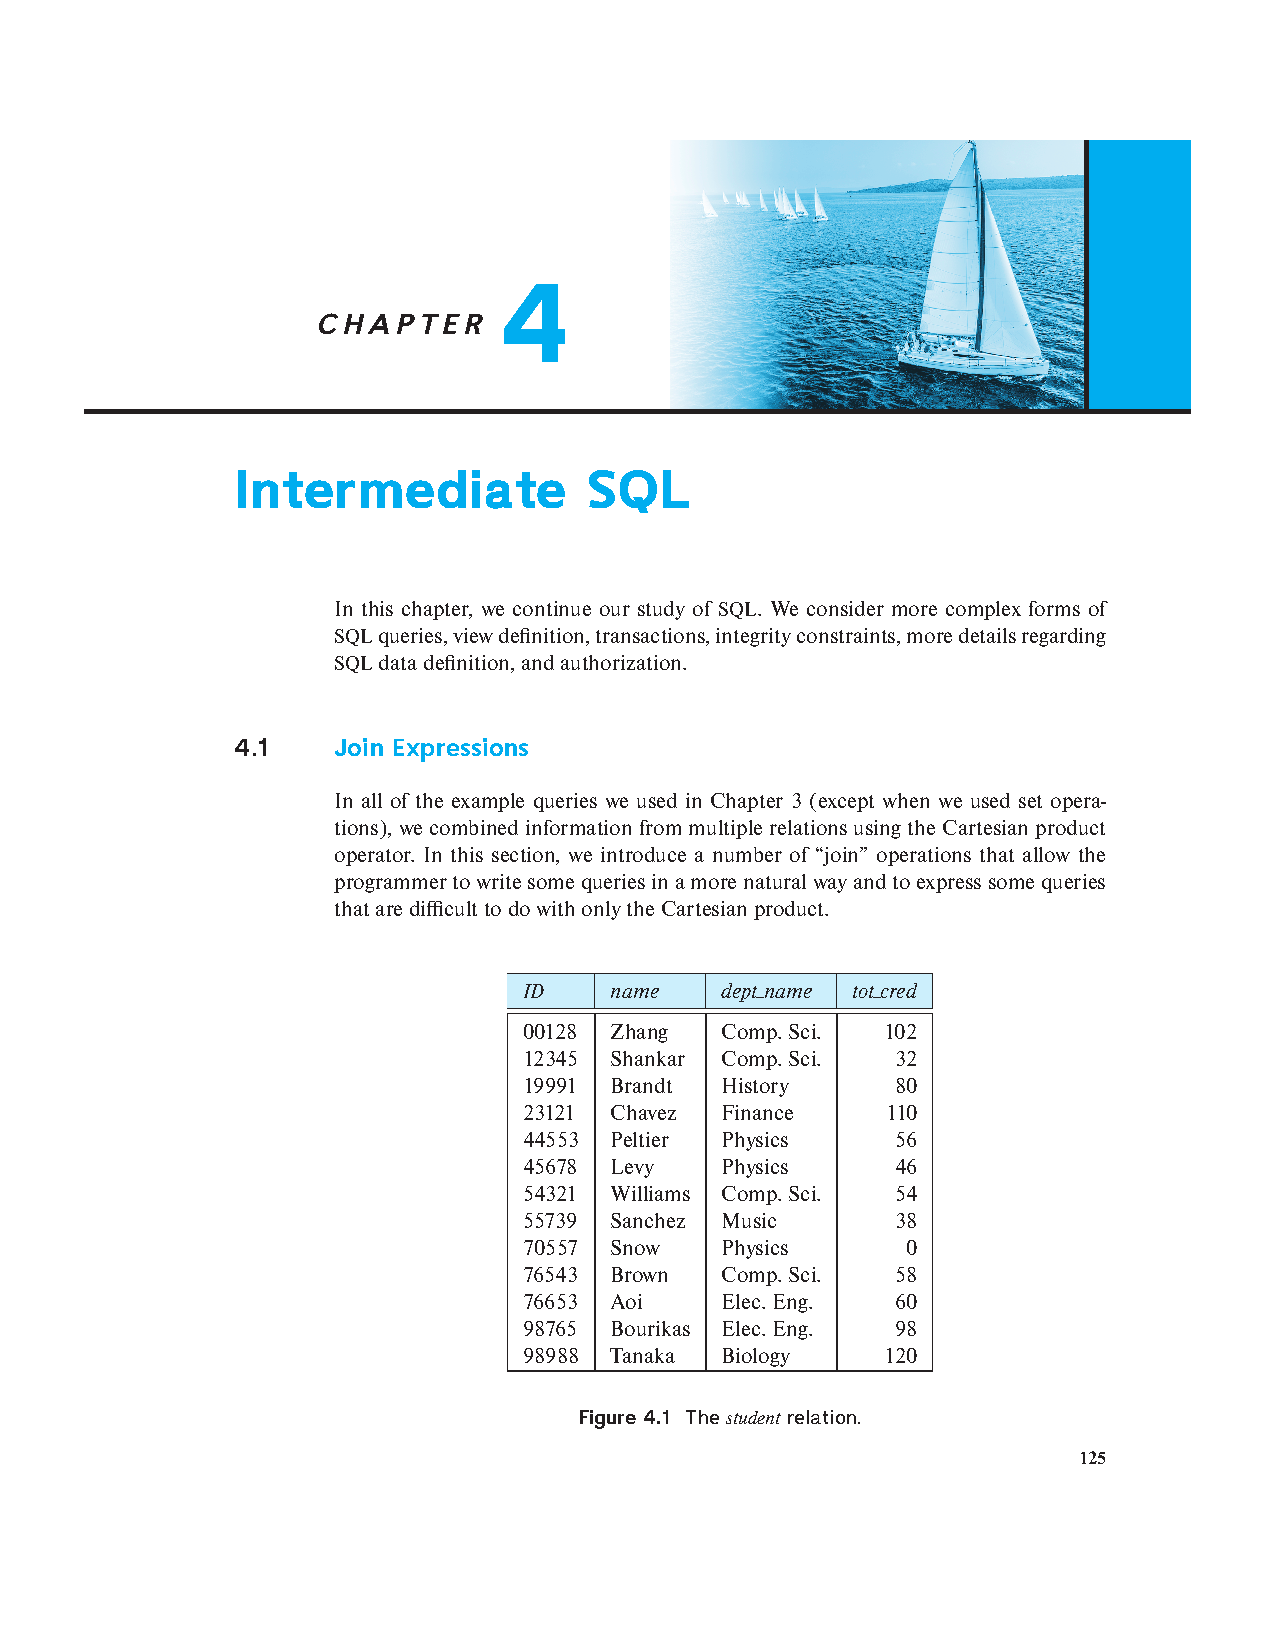
\includegraphics[width=0.75\textwidth, trim={8cm 4.5cm 5cm 16cm}, clip]{pages/nj1.pdf}
\end{frame}

\begin{frame}{Takes Relation}
    \centering
    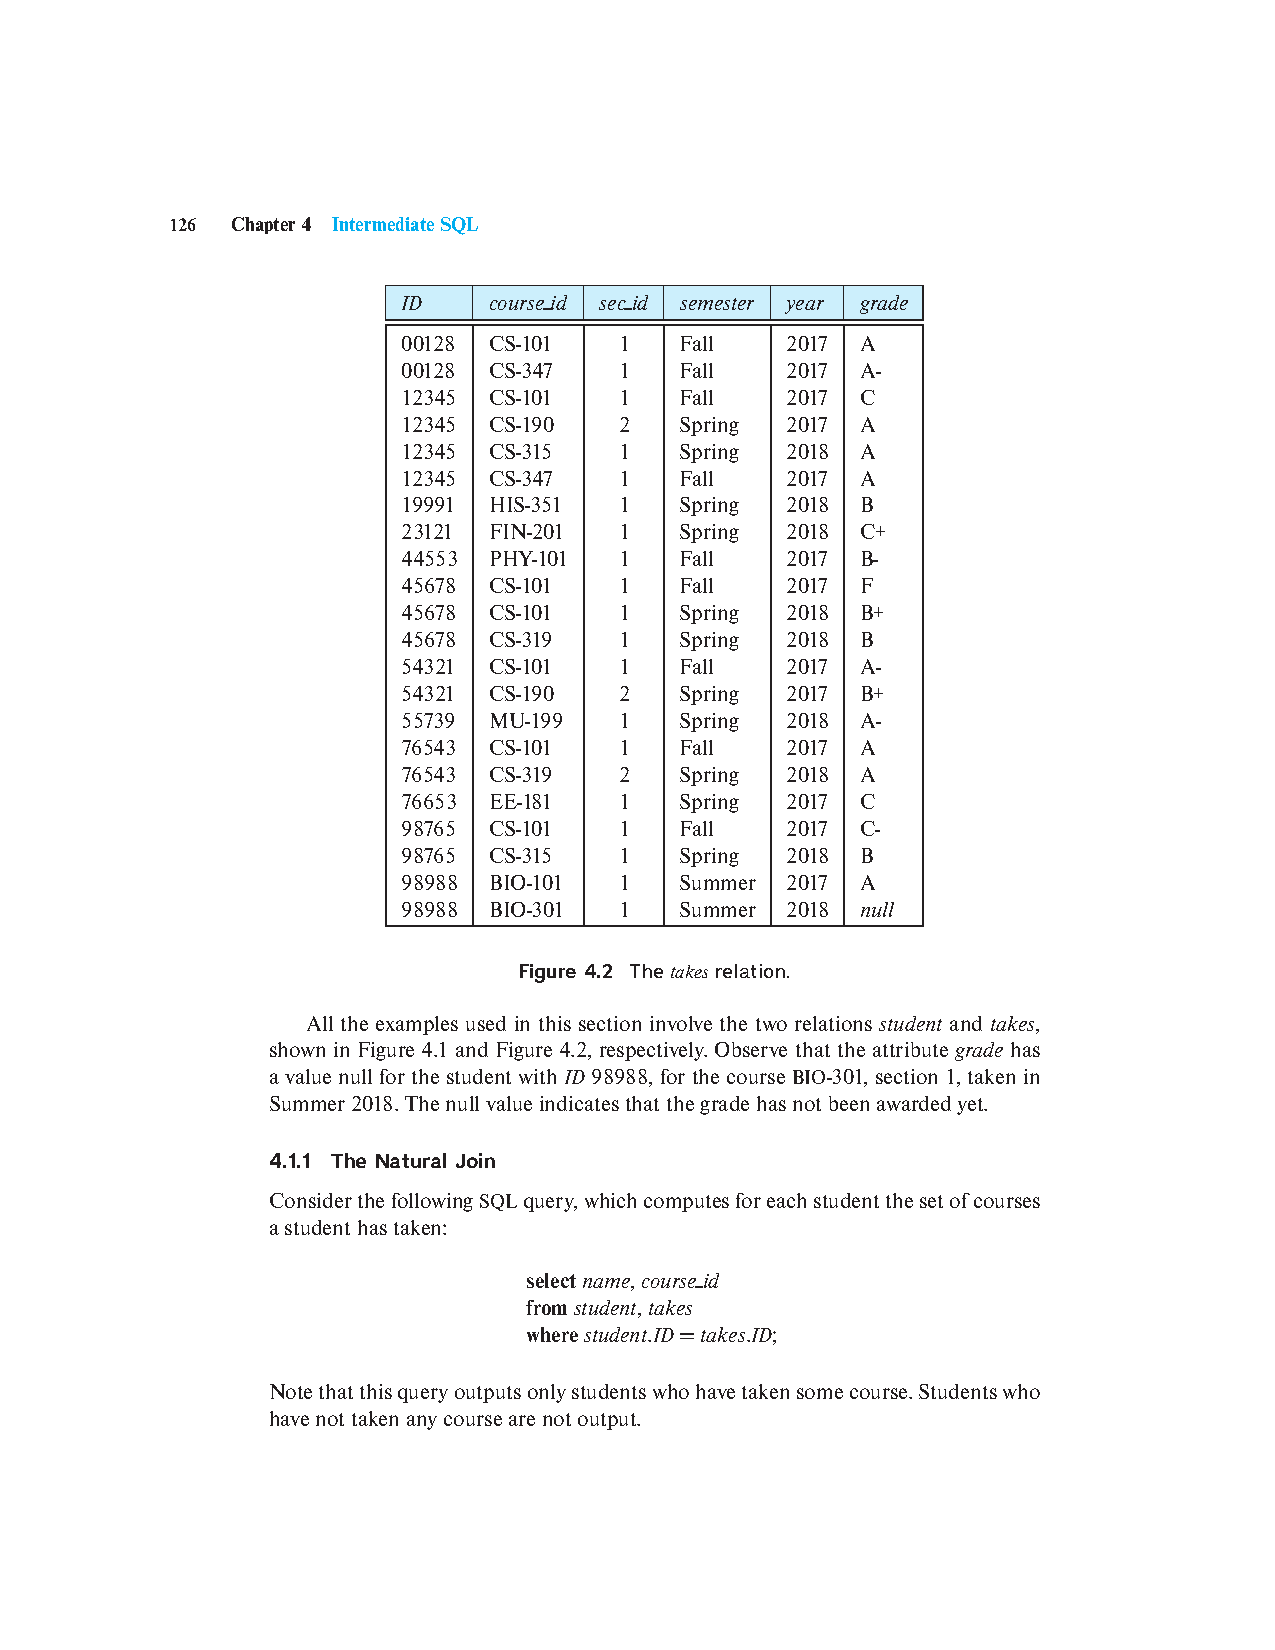
\includegraphics[width=0.75\textwidth, trim={4.5cm 12cm 5.5cm 4.5cm}, clip]{pages/nj2.pdf}
\end{frame}

\begin{frame}{Student Natural Join Takes}
    \centering
    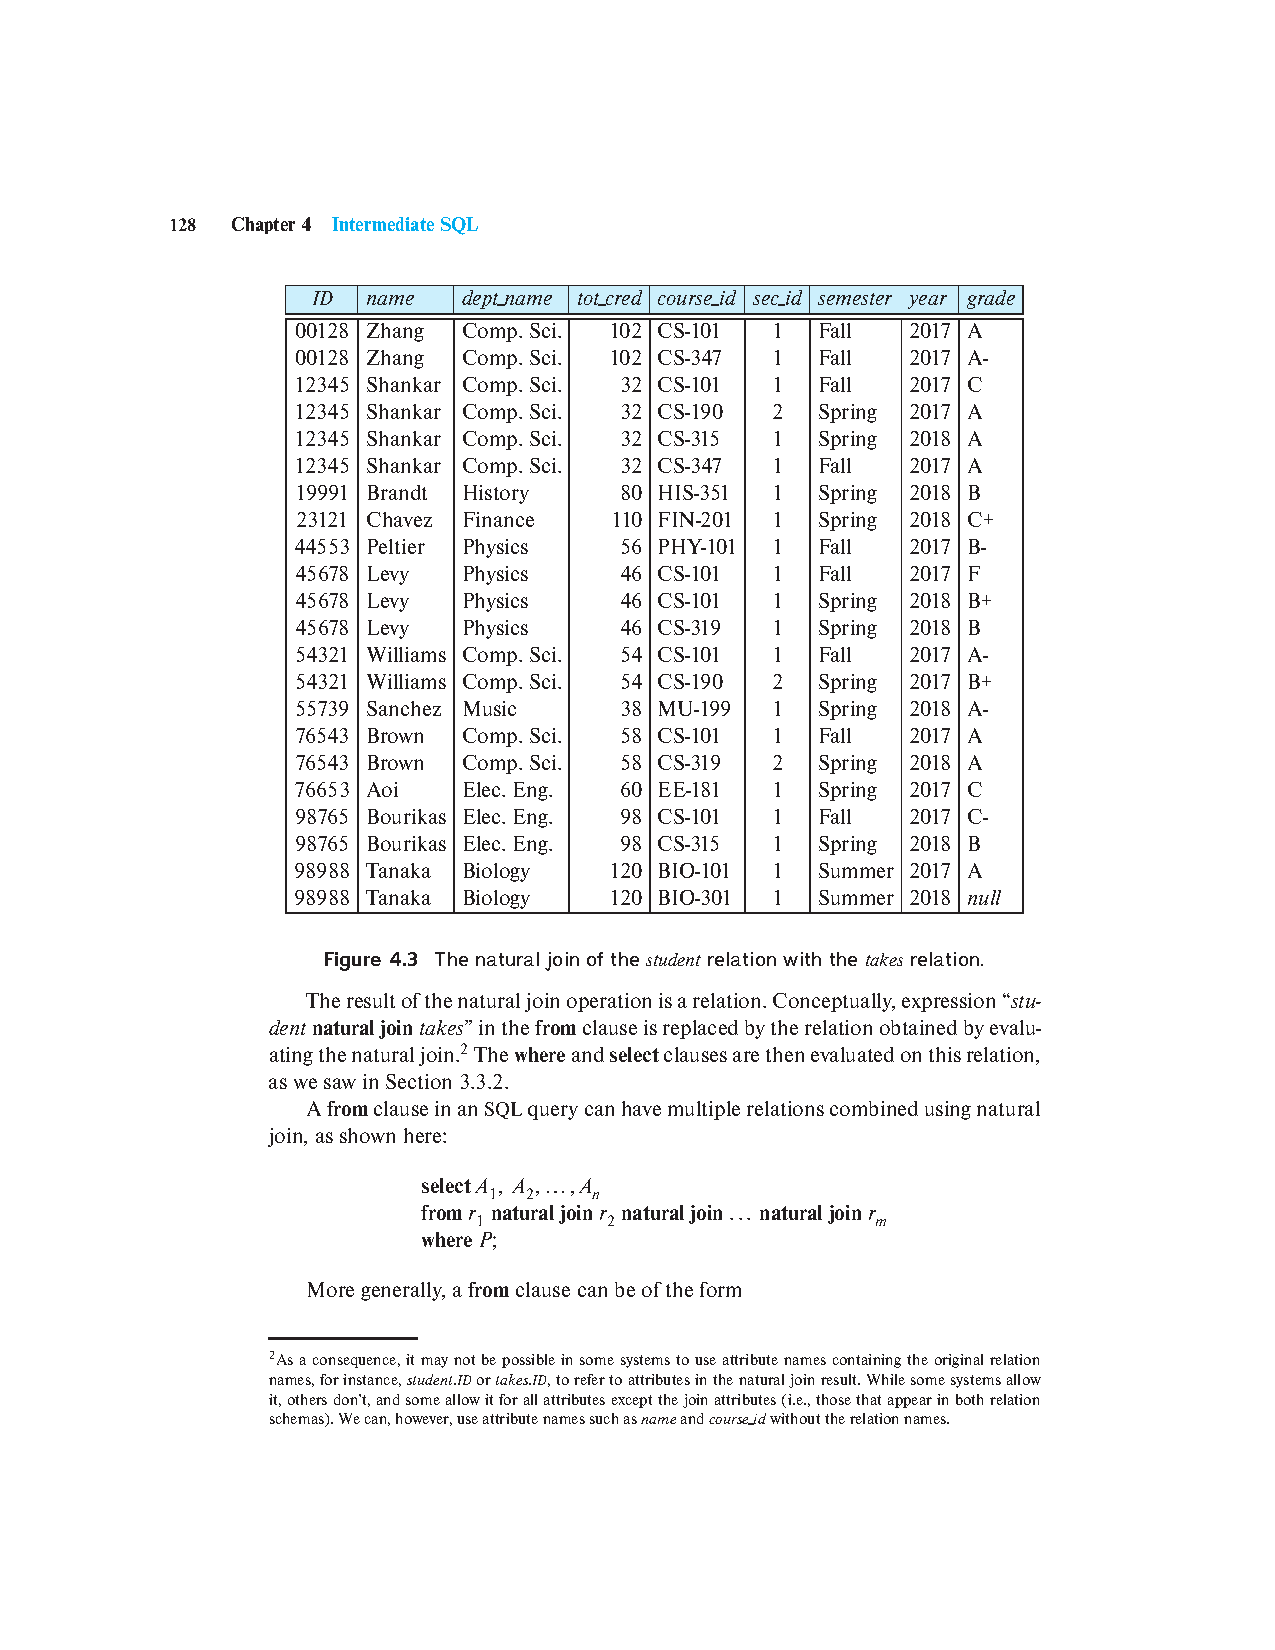
\includegraphics[width=0.95\textwidth, trim={3cm 12cm 3cm 4.5cm}, clip]{pages/nj3.pdf}
\end{frame}

\begin{frame}[fragile]{Dangerous in Natural Join}
    Beware of unrelated attributes with same name which get equated incorrectly
    \begin{exampleblock}{Example:}
        List the names of students along with the titles of courses that they have taken.
    \end{exampleblock}
    \begin{minted}
    [tabsize=4, obeytabs, frame=lines, framesep=2mm, baselinestretch=1.2, bgcolor=LightGray, fontsize=\footnotesize, linenos]{sql}
    SELECT
        name, title
    FROM
        student
    natural join
        takes
    natural join
        course;
    \end{minted}
    \pause
    \vspace{-5mm}
    \begin{FlushRight}
        \Large \textcolor{red}{\textbf{Incorrect!} {\footnotesize double check $dept\_name$ attribute}}
    \end{FlushRight}
\end{frame}

\begin{frame}[fragile]{Dangerous in Natural Join}
    \begin{exampleblock}{Example:}
        List the names of students along with the titles of courses that they have taken.
    \end{exampleblock}
    \begin{minted}
    [tabsize=4, obeytabs, frame=lines, framesep=2mm, baselinestretch=1.2, bgcolor=LightGray, fontsize=\scriptsize, linenos]{sql}
    SELECT
        name, title
    FROM
        student
    NATURAL JOIN
        takes
    NATURAL JOIN
        course;
    \end{minted}
    \vspace{-5mm}
    \begin{itemize}
        \item This query omits all (student name, course title) pairs where the student takes a course in a department other than the student's own department.
    \end{itemize}
\end{frame}

\begin{frame}[fragile]{Dangerous in Natural Join}
    \begin{exampleblock}{Example:}
        List the names of students along with the titles of courses that they have taken.
    \end{exampleblock}
    \begin{minted}
    [tabsize=4, obeytabs, frame=lines, framesep=2mm, baselinestretch=1.2, bgcolor=LightGray, fontsize=\scriptsize, linenos]{sql}
    SELECT
        name, title
    FROM
        student
    NATURAL JOIN
        takes, course
    WHERE
        takes.course_id = course.course_id;
    \end{minted}
    \vspace{-5mm}
    \begin{itemize}
        \item The correct version (above), correctly outputs such pairs.
    \end{itemize}
\end{frame}

\begin{frame}{Outer Join}
    \begin{itemize}
        \item An extension of the join operation that avoids loss of information.
        \item Computes the \texttt{JOIN} and then adds tuples form one relation that does not match tuples in the other relation to the result of the join.
        \item Uses \textbf{\texttt{null}} values.
        \item Three forms of outer join:
        \begin{itemize}
            \item left outer join
            \item right outer join
            \item full outer join
        \end{itemize}
    \end{itemize}
\end{frame}

\begin{frame}{Outer Join Examples}
    \begin{itemize}
        \item Relation \textit{course}: \\
            \vspace{2mm}
            \begin{tabular}{| l | l | l | c |}
                \hline
                \textbf{course\_id} & \textbf{title} & \textbf{dept\_name} & \textbf{credits} \\
                \hline
                BIO-301 & Genetics    & Biology    & 4 \\
                \hline
                CS-190  & Game Design & Comp. Sci. & 4 \\
                \hline
                CS-315  & Robotics    & Comp. Sci. & 3 \\
                \hline
            \end{tabular}
        \item Relation \textit{prereq}: \\
            \vspace{2mm}
            \begin{tabular}{| l | l |}
                \hline
                \textbf{course\_id} & \textbf{prereq\_id} \\
                \hline
                BIO-301 & BIO-101 \\
                \hline
                CS-190  & CS-101  \\
                \hline
                CS-347  & CS-101  \\
                \hline
            \end{tabular}
            \vspace{1mm}
        \item Observe that
        \begin{itemize}
            \item course information is missing for CS-347
            \item prereq information is missing for CS-315
        \end{itemize}
    \end{itemize}
\end{frame}

\begin{frame}{Left Outer Join}
    \begin{itemize}
        \item course \texttt{NATURAL LEFT OUTER JOIN} prereq
    \end{itemize}
    \vspace{5mm}
    \begin{tabular}{| l | l | l | c | l |}
        \hline
        \textbf{course\_id} & \textbf{title} & \textbf{dept\_name} & \textbf{credits} & \textbf{prereq\_id} \\
        \hline
        BIO-301 & Genetics    & Biology    & 4 & BIO-101 \\
        \hline
        CS-190  & Game Design & Comp. Sci. & 4 & CS-101  \\
        \hline
        CS-315  & Robotics    & Comp. Sci. & 3 & \textbf{\texttt{null}}\\
        \hline
    \end{tabular}
    \vspace{5mm}
    \begin{itemize}
        \item In relational algebra: course $\leftouterjoin$ prereq
    \end{itemize}
\end{frame}

\begin{frame}{Right Outer Join}
    \begin{itemize}
        \item course \texttt{NATURAL RIGHT OUTER JOIN} prereq
    \end{itemize}
    \vspace{5mm}
    \begin{tabular}{| l | l | l | c | l |}
        \hline
        \textbf{course\_id} & \textbf{title} & \textbf{dept\_name} & \textbf{credits} & \textbf{prereq\_id} \\
        \hline
        BIO-301 & Genetics    & Biology    & 4 & BIO-101 \\
        \hline
        CS-190  & Game Design & Comp. Sci. & 4 & CS-101  \\
        \hline
        CS-347  & \textbf{\texttt{null}}   & \textbf{\texttt{null}} & \textbf{\texttt{null}} & CS-101 \\
        \hline
    \end{tabular}
    \vspace{5mm}
    \begin{itemize}
        \item In relational algebra: course $\rightouterjoin$ prereq
    \end{itemize}
\end{frame}

\begin{frame}{Full Outer Join}
    \begin{itemize}
        \item course \texttt{NATURAL FULL OUTER JOIN} prereq
    \end{itemize}
    \vspace{5mm}
    \begin{tabular}{| l | l | l | c | l |}
        \hline
        \textbf{course\_id} & \textbf{title} & \textbf{dept\_name} & \textbf{credits} & \textbf{prereq\_id} \\
        \hline
        BIO-301 & Genetics    & Biology    & 4 & BIO-101 \\
        \hline
        CS-190  & Game Design & Comp. Sci. & 4 & CS-101  \\
        \hline
        CS-315  & Robotics    & Comp. Sci. & 3 & \textbf{\texttt{null}}\\
        \hline
        CS-347  & \textbf{\texttt{null}}   & \textbf{\texttt{null}} & \textbf{\texttt{null}} & CS-101 \\
        \hline
    \end{tabular}
    \vspace{5mm}
    \begin{itemize}
        \item In relational algebra: course $\fullouterjoin$ prereq
    \end{itemize}
\end{frame}

\begin{frame}{Joined Types and Conditions}
    \begin{itemize}
        \item \textbf{Join operations} – take two relations and return as a result another relation.
        \item These additional operations are typically used as subquery expressions in the \texttt{FROM} clause
        \item \textbf{Join condition} – defines which tuples in the two relations match, and what attributes are present in the result of the join.
        \item \textbf{Join type} – defines how tuples in each relation that do not match any tuple in the other relation (based on the join condition) are treated.
    \end{itemize}
    \centering
    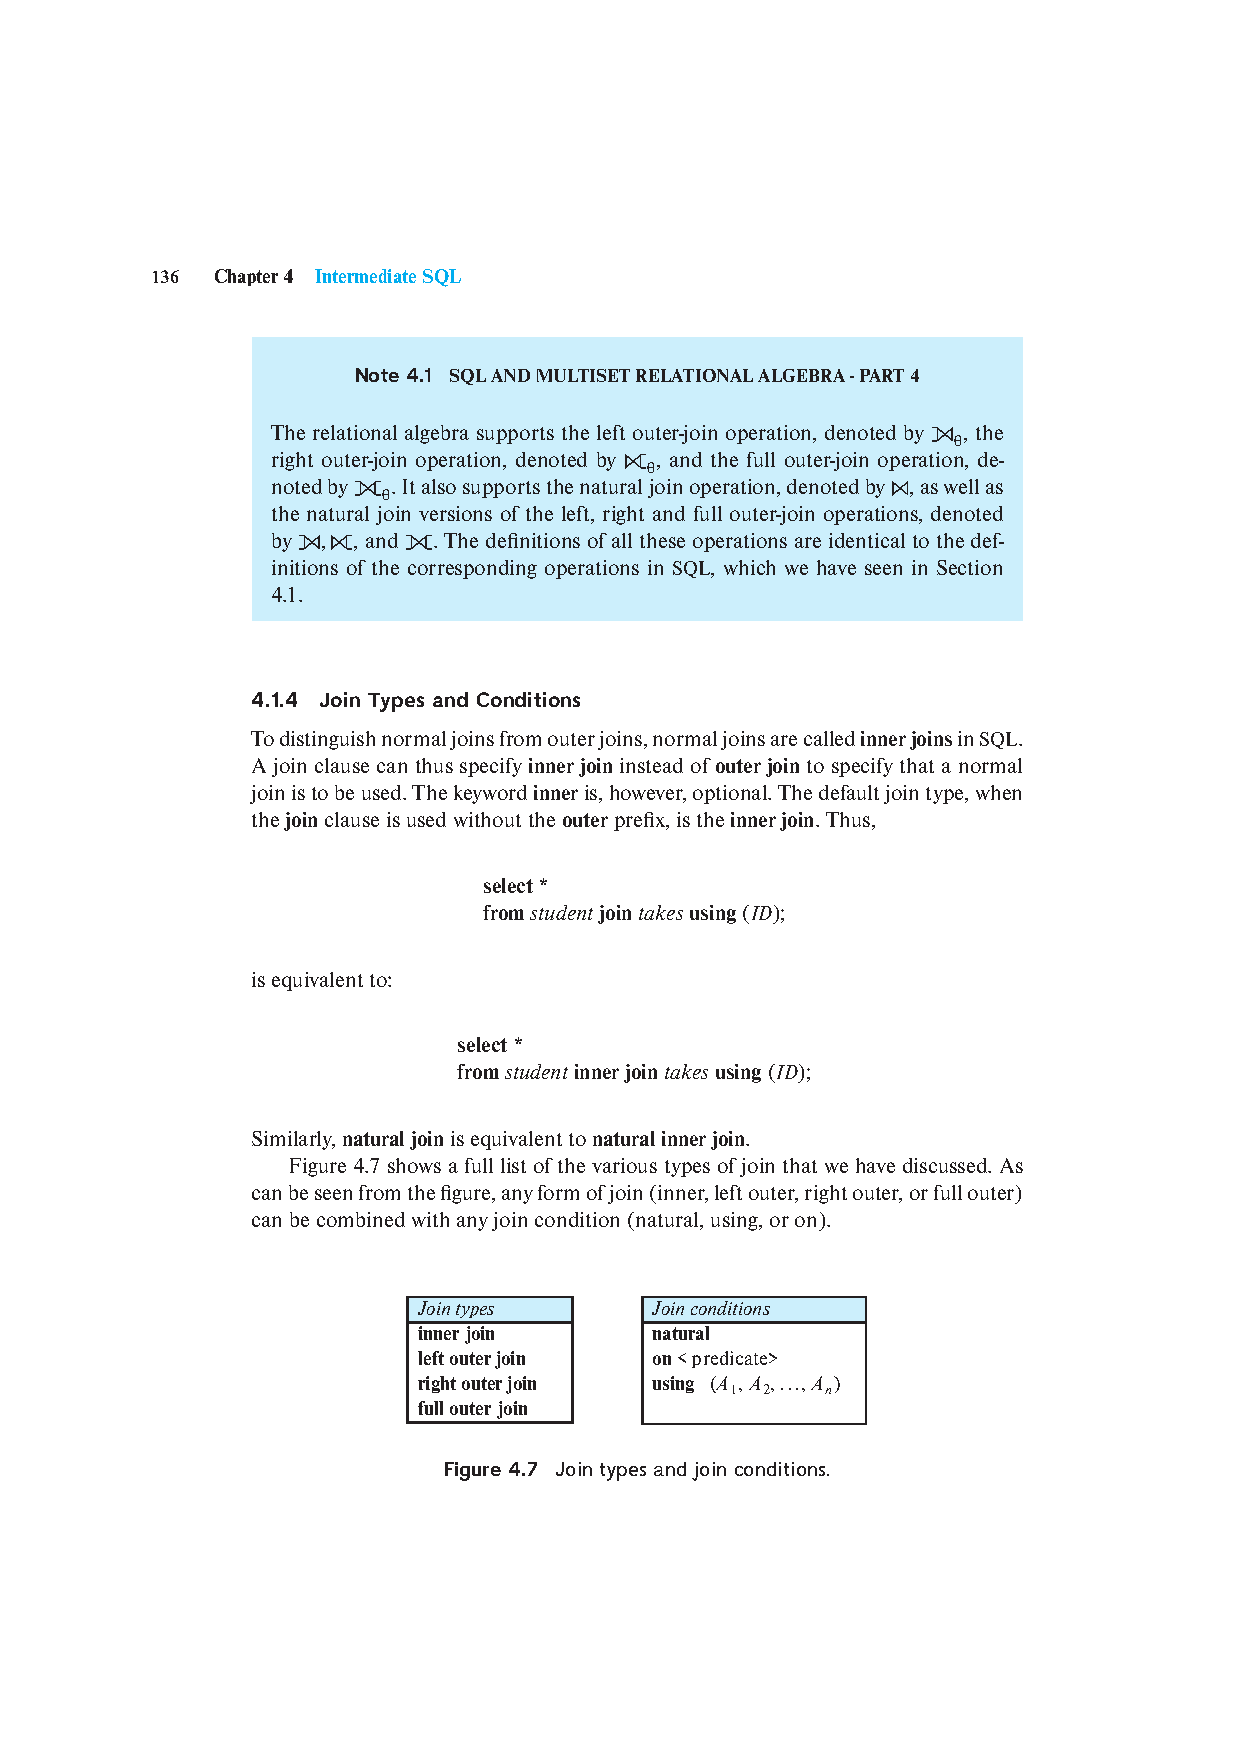
\includegraphics[width=\textwidth, trim={5cm 5.5cm 5cm 21.5cm}, clip]{pages/joins.pdf}
\end{frame}

\begin{frame}{Joined Relations – Examples}
    \begin{itemize}
        \item course \texttt{NATURAL RIGHT OUTER JOIN} prereq
    \end{itemize}
    \scriptsize
    \begin{tabular}{| l | l | l | c | l |}
        \hline
        \textbf{course\_id} & \textbf{title} & \textbf{dept\_name} & \textbf{credits} & \textbf{prereq\_id} \\
        \hline
        BIO-301 & Genetics    & Biology    & 4 & BIO-101 \\
        \hline
        CS-190  & Game Design & Comp. Sci. & 4 & CS-101  \\
        \hline
        CS-347  & \textbf{\texttt{null}}   & \textbf{\texttt{null}} & \textbf{\texttt{null}} & CS-101 \\
        \hline
    \end{tabular}
    \vspace{5mm}
    \normalsize
    \begin{itemize}
        \item course \texttt{FULL OUTER JOIN} prereq \texttt{USING} (course\_id)
    \end{itemize}
    \scriptsize
    \begin{tabular}{| l | l | l | c | l |}
        \hline
        \textbf{course\_id} & \textbf{title} & \textbf{dept\_name} & \textbf{credits} & \textbf{prereq\_id} \\
        \hline
        BIO-301 & Genetics    & Biology    & 4 & BIO-101 \\
        \hline
        CS-190  & Game Design & Comp. Sci. & 4 & CS-101  \\
        \hline
        CS-315  & Robotics    & Comp. Sci. & 3 & \textbf{\texttt{null}}\\
        \hline
        CS-347  & \textbf{\texttt{null}}   & \textbf{\texttt{null}} & \textbf{\texttt{null}} & CS-101 \\
        \hline
    \end{tabular}
\end{frame}

\begin{frame}{Joined Relations – Examples}
    \normalsize
    \begin{itemize}
        \item course \texttt{INNER JOIN} prereq \texttt{ON} course.course\_id = prereq.course\_id
    \end{itemize}
    \scriptsize
    \begin{tabular}{| l | l | l | c | l | l |}
        \hline
        \textbf{course\_id} & \textbf{title} & \textbf{dept\_name} & \textbf{credits} & \textbf{prereq\_id} & \textbf{course\_id} \\
        \hline
        BIO-301 & Genetics    & Biology    & 4 & BIO-101 & BIO-301 \\
        \hline
        CS-190  & Game Design & Comp. Sci. & 4 & CS-101  & CS-190  \\
        \hline
    \end{tabular}
    \normalsize
    \begin{itemize}
        \item What is the difference between the above, and a natural join?
        \vspace{5mm}
        \item course \texttt{LEFT OUTER JOIN} prereq \texttt{ON} course.course\_id = prereq.course\_id
    \end{itemize}
    \scriptsize
    \begin{tabular}{| l | l | l | c | l | l |}
        \hline
        \textbf{course\_id} & \textbf{title} & \textbf{dept\_name} & \textbf{credits} & \textbf{prereq\_id} & \textbf{course\_id} \\
        \hline
        BIO-301 & Genetics    & Biology    & 4 & BIO-101 & BIO-301 \\
        \hline
        CS-190  & Game Design & Comp. Sci. & 4 & CS-101 & CS-190  \\
        \hline
        CS-315  & Robotics    & Comp. Sci. & 3 & \textbf{\texttt{null}} & \textbf{\texttt{null}} \\
        \hline
    \end{tabular}
\end{frame}

\begin{frame}{Joined Relations – Examples}
    \normalsize
    \begin{itemize}
        \item course \texttt{NATURAL RIGHT OUTER JOIN} prereq
    \end{itemize}
    \scriptsize
    \begin{tabular}{| l | l | l | c | l |}
        \hline
        \textbf{course\_id} & \textbf{title} & \textbf{dept\_name} & \textbf{credits} & \textbf{prereq\_id} \\
        \hline
        BIO-301 & Genetics    & Biology    & 4 & BIO-101 \\
        \hline
        CS-190  & Game Design & Comp. Sci. & 4 & CS-101  \\
        \hline
        CS-347  & \texttt{\textbf{null}} & \texttt{\textbf{null}} & \texttt{\textbf{null}} & CS-101  \\
        \hline
    \end{tabular}
    \vspace{5mm}
    \normalsize
    \begin{itemize}
        \item course \texttt{FULL OUTER JOIN} prereq \texttt{USING} (course\_id)
    \end{itemize}
    \scriptsize
    \begin{tabular}{| l | l | l | c | l |}
        \hline
        \textbf{course\_id} & \textbf{title} & \textbf{dept\_name} & \textbf{credits} & \textbf{prereq\_id} \\
        \hline
        BIO-301 & Genetics    & Biology    & 4 & BIO-101 \\
        \hline
        CS-190  & Game Design & Comp. Sci. & 4 & CS-101  \\
        \hline
        CS-315  & Robotics    & Comp. Sci. & 3 & \textbf{\texttt{null}} \\
        \hline
        CS-347  & \texttt{\textbf{null}} & \texttt{\textbf{null}} & \texttt{\textbf{null}} & CS-101  \\
        \hline
    \end{tabular}
\end{frame}

\section{Views}

\begin{frame}[fragile]{Views}
    \begin{itemize}
        \item In some cases, it is not desirable for all users to see the entire logical model (that is, all the actual relations stored in the database.)
        \item Consider a person who needs to know an instructors name and department, but not the salary. This person should see a relation described, in \texttt{SQL}, by
        \begin{minted}
        [tabsize=4, obeytabs, frame=lines, framesep=2mm, baselinestretch=1.2, bgcolor=LightGray, fontsize=\scriptsize, linenos]{sql}
    SELECT
        ID, name, dept_name
    FROM
        instructor;
        \end{minted}
        \item A \textcolor{blue}{\textbf{view}} provides a mechanism to hide certain data from the view of certain users.
        \item Any relation that is not of the conceptual model but is made visible to a user as a “virtual relation” is called a \textbf{\textcolor{blue}{view}}.
    \end{itemize}
\end{frame}

\begin{frame}[fragile]{View Definition}
    \begin{itemize}
        \item A view is defined using the create view statement which has the form:
            \begin{lstlisting}[language=SQL]
    CREATE VIEW v AS @($< query\_expression >$)@;
            \end{lstlisting}
            where $<query\_expression>$ is any legal \texttt{SQL} expression. The view name is represented by v.
        \item Once a view is defined, the view name can be used to refer to the virtual relation that the view generates.
        \item View definition is not the same as creating a new relation by evaluating the query expression
            \begin{itemize}
                \item Rather, a view definition causes the saving of an expression; the expression is substituted into queries using the view.
            \end{itemize}
    \end{itemize}
\end{frame}

\begin{frame}[fragile]{View Definition and Use}
    \begin{itemize}
        \item A view of instructors without their salary.
    \end{itemize}
    \begin{minted}
    [tabsize=4, obeytabs, frame=lines, framesep=2mm, baselinestretch=1.2, bgcolor=LightGray, fontsize=\scriptsize, linenos]{sql}
    CREATE VIEW faculty AS
    SELECT ID, name, dept_name
    FROM instructor
    \end{minted}
    \pause
    \vspace{-5mm}
    \begin{itemize}
        \item Find all instructors in the Biology department
    \end{itemize}
    \begin{minted}
    [tabsize=4, obeytabs, frame=lines, framesep=2mm, baselinestretch=1.2, bgcolor=LightGray, fontsize=\scriptsize, linenos]{sql}
    SELECT name
    FROM faculty
    WHERE dept_name = 'Biology'
    \end{minted}
    \pause
    \vspace{-5mm}
    \begin{itemize}
        \item Create a view of department salary totals
    \end{itemize}
    \begin{minted}
    [tabsize=4, obeytabs, frame=lines, framesep=2mm, baselinestretch=1.2, bgcolor=LightGray, fontsize=\scriptsize, linenos]{sql}
    CREATE VIEW departments_total_salary(dept_name, total_salary) AS
    SELECT dept_name, SUM(salary)
    FROM instructor
    GROUP BY dept_name;
    \end{minted}
\end{frame}

\begin{frame}{Views Defined Using Other Views}
    \begin{itemize}
        \item One view may be used in the expression defining another view.
        \item A view relation $v_1$ is said to \textcolor{blue}{depend directly} on a view relation $v_2$ if $v_2$ is used in the expression defining $v_1$.
        \item A view relation $v_1$ is said to \textcolor{blue}{depend on} view relation $v_2$ if either $v_1$ depends directly to $v_2$ or there is a path of dependencies from $v_1$ to $v_2$.
        \item A view relation $v$ is said to be \textcolor{blue}{recursive} if it depends on itself.
    \end{itemize}
\end{frame}

\begin{frame}[fragile]{Views Defined Using Other Views}
    \begin{minted}
    [tabsize=4, obeytabs, frame=lines, framesep=2mm, baselinestretch=1.2, bgcolor=LightGray, fontsize=\footnotesize, linenos]{sql}
    CREATE VIEW
        physics_fall_2017 AS
    SELECT
        course.course_id, sec_id, building, room_number
    FROM
        course, section
    WHERE
        course.course_id = section.course_id AND
        course.dept_name = 'Physics' AND
        section.semester = 'Fall' AND
        section.year = '2017';
    \end{minted}
\end{frame}

\begin{frame}[fragile]{Views Defined Using Other Views}
    \begin{minted}
    [tabsize=4, obeytabs, frame=lines, framesep=2mm, baselinestretch=1.2, bgcolor=LightGray, fontsize=\footnotesize, linenos]{sql}
    CREATE VIEW
        physics_fall_2017_watson AS
    SELECT
        course_id, room_number
    FROM
        physics_fall_2017
    WHERE
        building= 'Watson';
    \end{minted}
\end{frame}

\begin{frame}[fragile]{View Expansion}
    \begin{itemize}
        \item Expand the view:
            \begin{minted}
            [tabsize=4, obeytabs, frame=lines, framesep=2mm, baselinestretch=1.2, bgcolor=LightGray, fontsize=\scriptsize, linenos]{sql}
CREATE VIEW physics_fall_2017_watson AS
    SELECT course_id, room_number
    FROM physics_fall_2017
    WHERE building= 'Watson';
            \end{minted}
        \item To:
            \begin{minted}
            [tabsize=4, obeytabs, frame=lines, framesep=2mm, baselinestretch=1.2, bgcolor=LightGray, fontsize=\scriptsize, linenos]{sql}
CREATE VIEW physics_fall_2017_watson AS
    SELECT course_id, room_number
    FROM ( SELECT course.course_id, sect_id, building, room_number
            FROM course, section
            WHERE course.course_id = section.course_id
            AND course.dept_name = 'Physics'
            AND section.semester = 'Fall'
            AND section.year = '2017' )
    WHERE building= 'Watson';
            \end{minted}
    \end{itemize}
\end{frame}

\begin{frame}[fragile]{View Expansion (Cont.)}
    \begin{itemize}
        \item A way to define the meaning of views defined in terms of other views.
        \item Let view $v_1$ be defined by an expression $e_1$ that may itself contain uses of view relations.
        \item View expansion of an expression repeats the following replacement step:
            \footnotesize
            \begin{lstlisting}[language=bash]
REPEAT
    Find any view relation @($v_i$)@ in @($e_i$)@
    Replace the view relation @($v_i$)@
        by the expression defining @($v_i$)@
UNTIL no more view relations are present in @($e_i$)@
            \end{lstlisting}
            \normalsize
        \item As long as the view definitions are not recursive, this loop will terminate.
    \end{itemize}
\end{frame}

\begin{frame}{Materialized Views}
    \begin{itemize}
        \item Certain database systems allow view relations to be physically stored.
            \begin{itemize}
                \item Physical copy created when the view is defined.
                \item Such views are called \textbf{\textcolor{blue}{Materialized view}}.
            \end{itemize}
        \item If relations used in the query are updated, the materialized view result becomes out of date.
            \begin{itemize}
                \item Need to \textcolor{blue}{\textbf{maintain}} the view, by updating the view whenever the underlying relations are updated.
            \end{itemize}
    \end{itemize}
\end{frame}

\begin{frame}[fragile]{Update of a View}
    \begin{itemize}
        \item Add a new tuple to faculty view which we defined earlier.
            \begin{minted}
            [tabsize=4, obeytabs, frame=lines, framesep=2mm, baselinestretch=1.2, bgcolor=LightGray, fontsize=\scriptsize]{sql}
    INSERT INTO faculty
    VALUES ('30765', 'Green', 'Music');
            \end{minted}
        \item This insertion must be represented by the insertion into the instructor relation.
            \begin{itemize}
                \item Must have a value for salary.
            \end{itemize}
        \item Two approaches:
            \begin{itemize}
                \item Reject the insert.
                \item Insert the tuple:\\
                    \texttt{(`30765', `Green', `Music', \textbf{null})}\\
                    into the \textit{instructor} relation.
            \end{itemize}
    \end{itemize}
\end{frame}

\begin{frame}[fragile]{Some Updates Cannot be Translated Uniquely}
    \begin{itemize}
        \item[ ]
        \begin{minted}
        [tabsize=4, obeytabs, frame=lines, framesep=2mm, baselinestretch=1.2, bgcolor=LightGray, fontsize=\scriptsize]{sql}
CREATE VIEW instructor_info AS
    SELECT
        ID, name, building
    FROM
        instructor, department
    WHERE
        instructor.dept_name= department.dept_name;
        \end{minted}
        \item[ ]
        \vspace{-7mm}
        \begin{minted}
        [tabsize=4, obeytabs, frame=lines, framesep=2mm, baselinestretch=1.2, bgcolor=LightGray, fontsize=\scriptsize]{sql}
INSERT INTO instructor_info
VALUES ('69987', 'White', 'Taylor');
        \end{minted}
        \item Issues:
            \begin{itemize}
                \item Which department, if multiple departments in Taylor?
                \item What if no department is in Taylor?
            \end{itemize}
    \end{itemize}
\end{frame}

\begin{frame}[fragile]{And Some Not at All}
    \begin{itemize}
        \item[ ]
        \begin{minted}
        [tabsize=4, obeytabs, frame=lines, framesep=2mm, baselinestretch=1.2, bgcolor=LightGray, fontsize=\scriptsize]{sql}
CREATE VIEW history_instructors AS
    SELECT *
    FROM instructor
    WHERE dept_name= 'History';
        \end{minted}
        \item What happens if we insert:\\
                \texttt{(`25566', `Brown', `Biology', 100000)}\\
                into \textit{history\_instructors}?
    \end{itemize}
\end{frame}

\begin{frame}{View Updates in SQL}
    \begin{itemize}
        \item Most \texttt{SQL} implementations allow updates only on simple views:
        \begin{itemize}
            \item The \texttt{FROM} clause has only one database relation.
            \item The \texttt{SELECT} clause contains only attribute names of the relation, and does not have any expressions, aggregates, or distinct specification.
            \item Any attribute not listed in the \texttt{SELECT} clause can be set to \texttt{\textbf{null}}.
            \item The query does not have a \texttt{GROUP BY} or \texttt{HAVING} clause.
        \end{itemize}
    \end{itemize}
\end{frame}










\section{Transactions}
\section{Integrity Constraints}
\section{SQL Data Types and Schemas}
\section{Index Definition in SQL}
\section{Authorization}

\begin{frame}[fragile]{}
    \begin{minted}
    [tabsize=4, obeytabs, frame=lines, framesep=2mm, baselinestretch=1.2, bgcolor=LightGray, fontsize=\footnotesize, linenos]{sql}
    \end{minted}
\end{frame}

\begin{frame}{}
\end{frame}

% \begin{frame}{}
%      \centering
%      \Huge End of Chapter 4.
% \end{frame}

% \section*{Takeaways}
% 
% % Tim Duncan's Top 5 Fundamental Takeaways of the Today's Class
% \begin{frame}{TDT5FTOTTC}
%     \centering
%     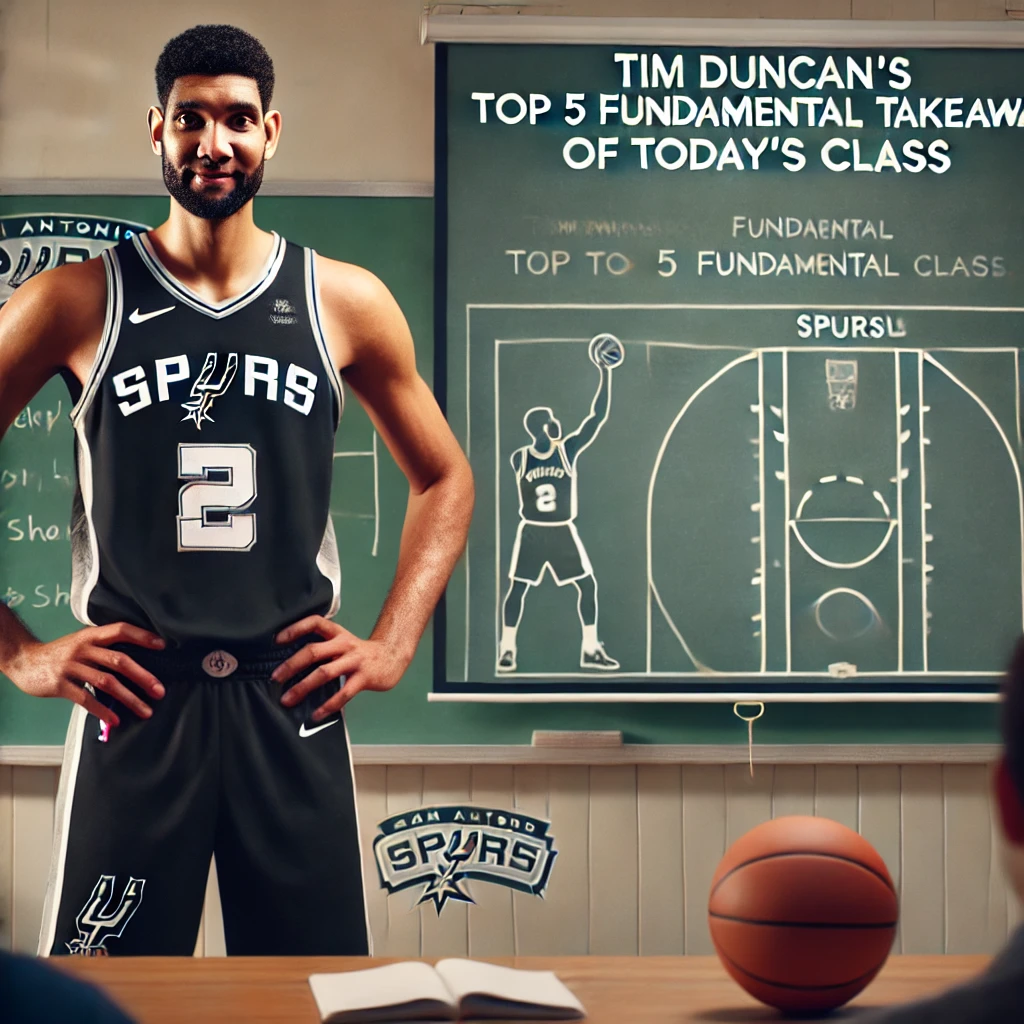
\includegraphics[width=0.75\textwidth]{figures/tim.png}
% \end{frame}
% 
% \begin{frame}{Top 5 Fundamental Takeaways}
%     \small
%     \begin{enumerate} \pause
%         \item[5] \textbf{}. \pause
%         \item[4] \textbf{}. \pause
%         \item[3] \textbf{}. \pause
%         \item[2] \textbf{}. \pause
%         \item[1] \textbf{}.
%     \end{enumerate}
% \end{frame}

\begin{frame}{Database System Concepts}
    \centering
    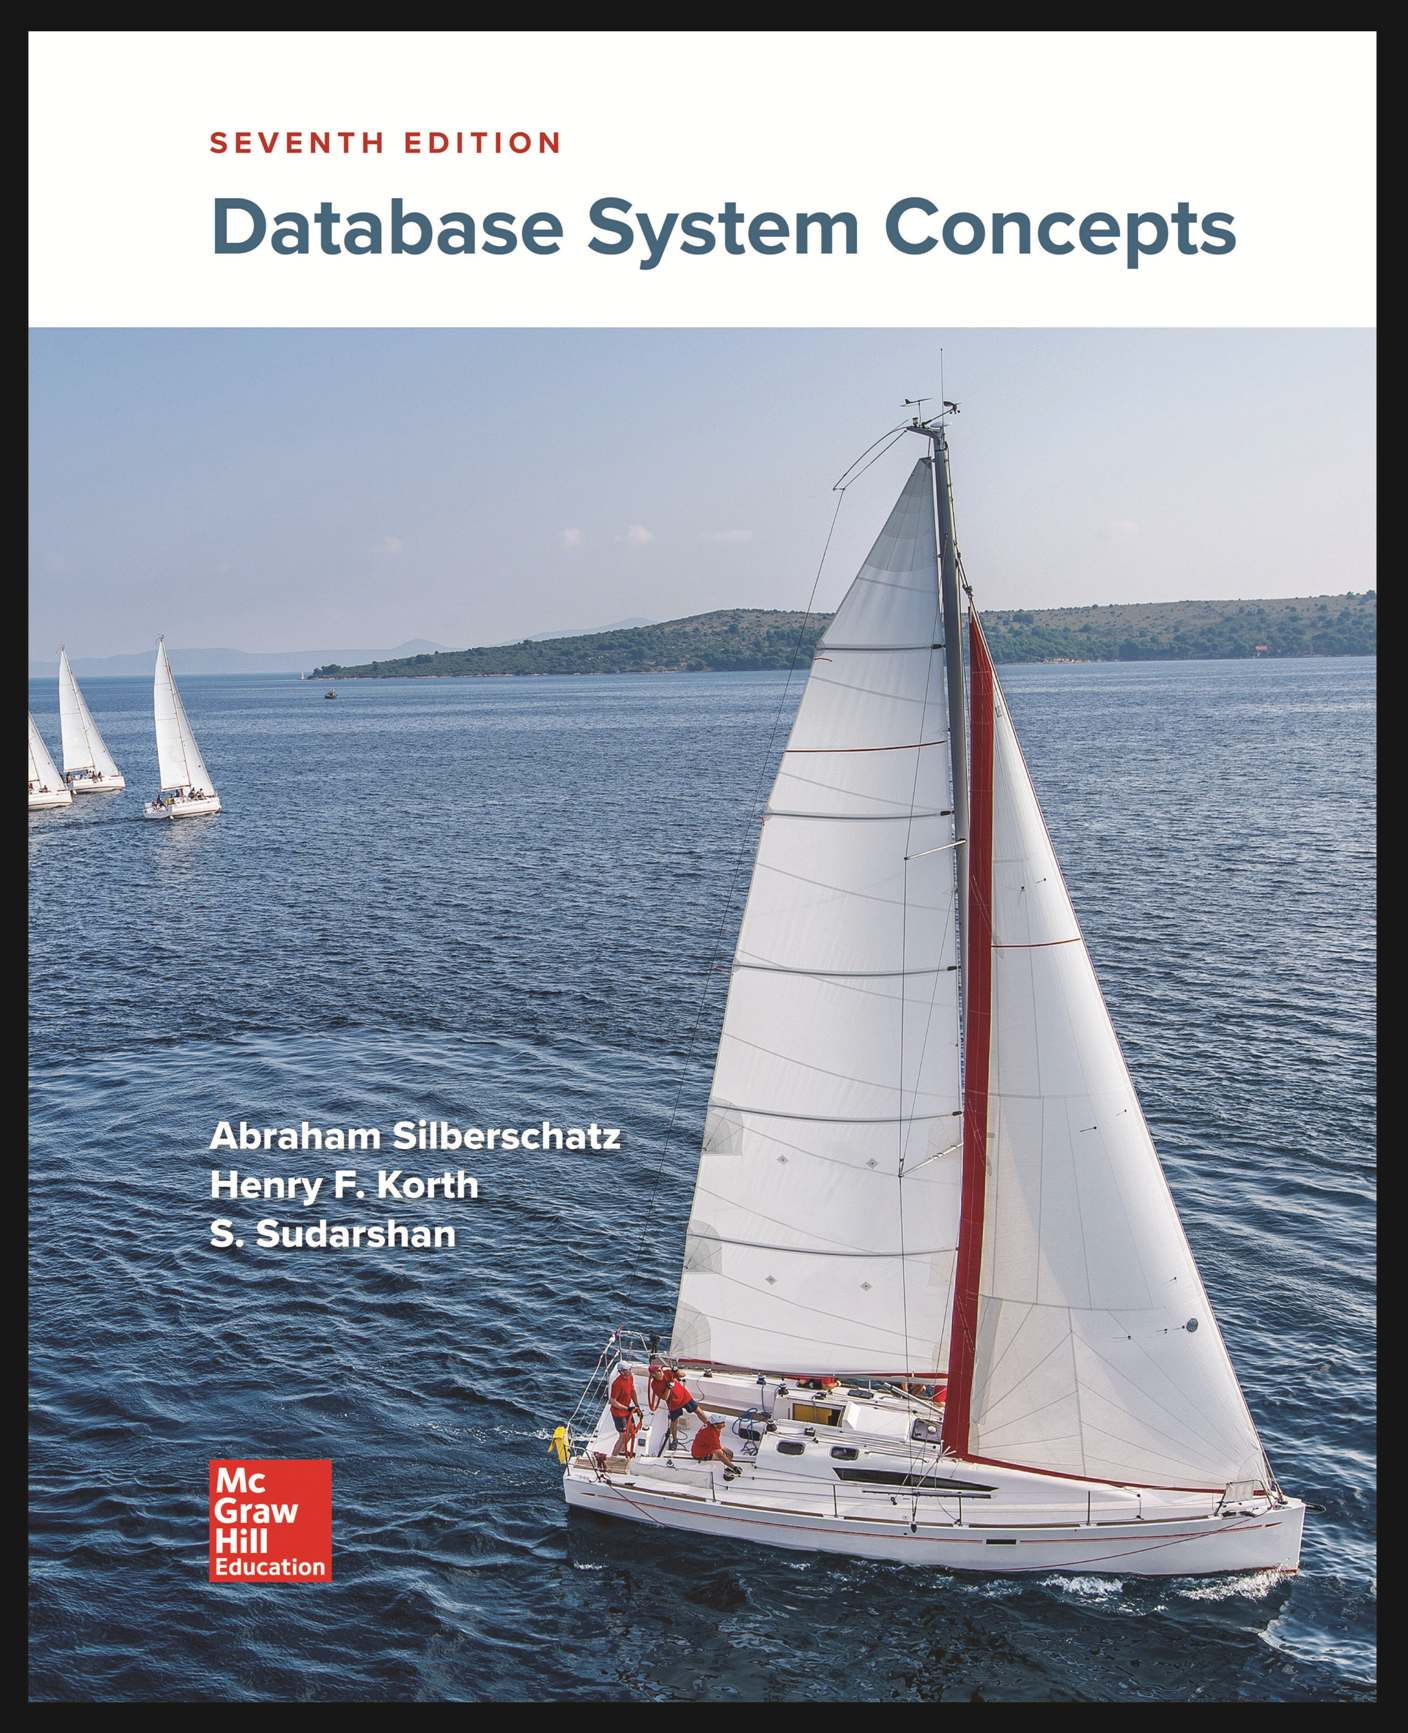
\includegraphics[width=0.5\textwidth]{figures/book_cover.jpg} \\
    \vspace{5mm}
    {
        \tiny
        Content has been extracted from \textit{Database System Concepts}, Seventh Edition, by Silberschatz, Korth and Sudarshan. Mc Graw Hill Education. 2019.\\
        Visit \url{https://db-book.com/}.\\
    }
\end{frame}

\end{document}
